\documentclass{article}

\usepackage[latin1]{inputenc}  
\usepackage[export]{adjustbox}
\usepackage{graphicx}
\graphicspath{ {image/} }

\makeatletter
\def\thickhrulefill{\leavevmode \leaders \hrule height 1pt\hfill \kern \z@}
\renewcommand{\maketitle}{\begin{titlepage}%
    \let\footnotesize\small
    \let\footnoterule\relax
    \parindent \z@
    \reset@font
    \null
    \vskip 50\p@
    \begin{center}
      \hrule height 1pt
      \vskip 1pt 
      \hrule
      \vskip 3pt
      {\huge \bfseries \strut \@title \strut}\par
      \vskip 1pt
      \hrule
      \vskip 1pt
      \hrule height 1pt
    \end{center}
    \vskip 50\p@
    \begin{flushright}
      \Large \@author \par
    \end{flushright}
    \vfil
    \null
    
  \end{titlepage}%
  \setcounter{footnote}{0}%
}

\title{Rapport Projet IDM}
\date{30 09 2016}
\author{Wargnier Pierre}

\begin{document}
		
\pagenumbering{gobble}
\maketitle
\newpage
\pagenumbering{arabic}
  
\section{Section}
  
  H\'ello World!
  
\subsection{Subsection}

\begin{figure}[h]

  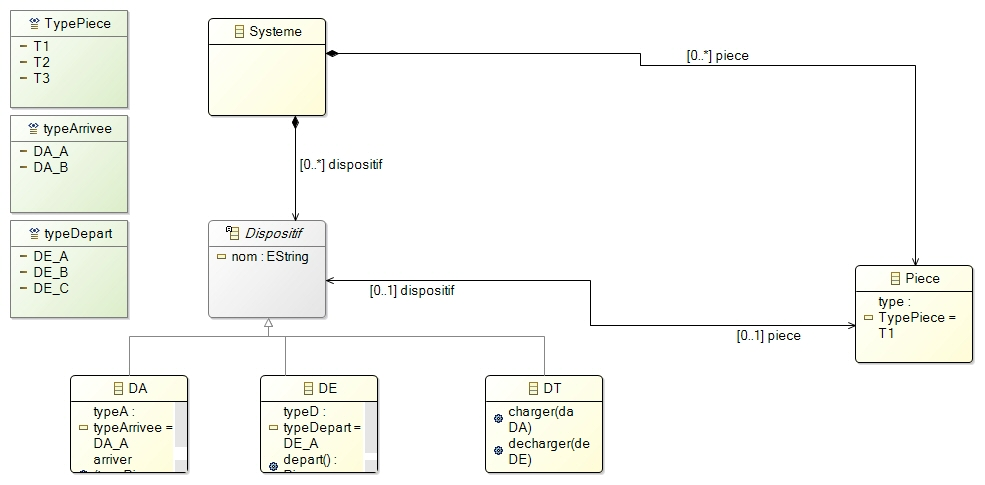
\includegraphics[width=500pt,center]{classDiagram.jpg}
  \centering{Voici le diagramme de classe}
  \label{fig:boat1}
\end{figure}

Structuring a document is easy!

\subsubsection{Subsubsection}

More text.

\paragraph{Paragraph}

Some more text.

\subparagraph{Subparagraph}

Even more text.

\section{Another section}
\pagenumbering{arabic}

Hello World!

\end{document}